\chapter{Pruebas}
En este capítulo vamos a presentar las diferentes pruebas y la experimentación
realizada con los algoritmos implementados

\section{Pruebas}
En primer lugar, vamos a comentar las pruebas realizadas a cada algoritmo
para confirmar su correcto funcionamiento y para observar con más claridad
su comportamiento. Para ello todos los algoritmos han sido probados con un
conjunto de datos sintéticos. Este conjunto de datos se ha generado haciendo
uso del generador de numpy de números aleatorios. Para generar un conjunto
de datos con anomalías hemos usado una distribución estándar y hemos generado 
100 puntos de dimensión 2. Este conjunto de puntos se distribuye uniformemente
en la distribución seleccionada. Para generar anomalías vamos a generar 20
puntos que rompan con esta distribución. Para ello estos 20 puntos de dimensión
2 los generamos con una distribución uniforme. De este modo aseguramos que los 
los 20 puntos tienen una distribución diferente y podremos usarlos con anomalías.

Para ver el comportamiento de cada algoritmo vamos a mostrar los datos y 
alrededor de cada punto mostraremos un radio en función del score asignado a
cada punto. Para tener una medida más exacta y numérica de la efectividad del
algoritmo vamos a usar las curvas \textbf{ROC} y la métrica \textbf{AUC}.
Las curvas \textbf{ROC} enfrentan en una grafica la tasa de verdaderos
positicos $TPR$ con tra la tasa de falsos positivos $FPR$ donde ambos se definen como:

\[ TPR = \frac{VP}{VP + FN}\]

\[FPR = \frac{FP}{FP +VN}\]

La métrica \textbf{AUC} se cálcula como el área bajo la curva \textbf{ROC}. Proporciona 
una medición agregada del rendimiento en todos los umbrales de clasificación 
posibles. Una forma de interpretar el \textbf{AUC} es como la probabilidad de 
que el modelo clasifique un ejemplo positivo aleatorio más alto que un ejemplo 
negativo aleatorio.
Con esta métrica tenemos una medida muy eficiente del desempeño de nuestro
sistema ya que se tendrán en cuenta tanto los errores negativos como positivos.

También mencionar que se trata de un problema de clasificación desbalanceado por lo que
queremos poner el foco en la detección de las instancias anomalas sin aumentar la tasa
de falsos positivos.

En las siguientes figuras mostramos en primer lugar el desempeño observando el
radios. Para ver con más claridad los puntos que eran anomalías originalmente, 
estos están representados con un color diferente. Veamos el comportamiento de
los algoritmos implementados.




\begin{figure}[H]
    \begin{tabular}{cc}
      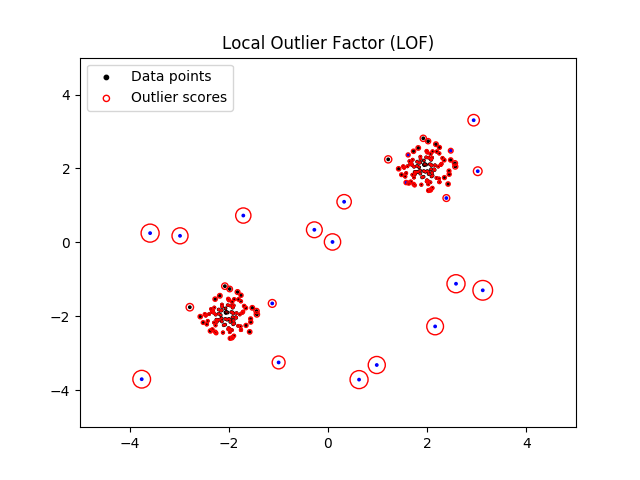
\includegraphics[width=65mm,height=40mm]{imagenes/lof-sintetico.png} &   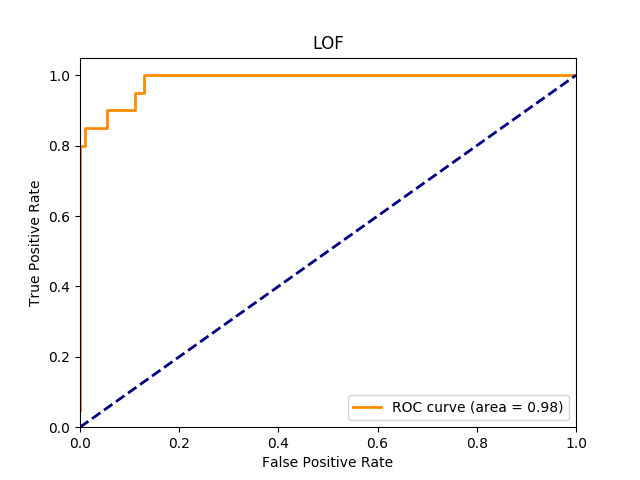
\includegraphics[width=65mm,height=40mm]{imagenes/lof-sintetic-roc.png} \\
    Score & Curca ROC para datos sinteticos \\[6pt]
    \multicolumn{2}{c}{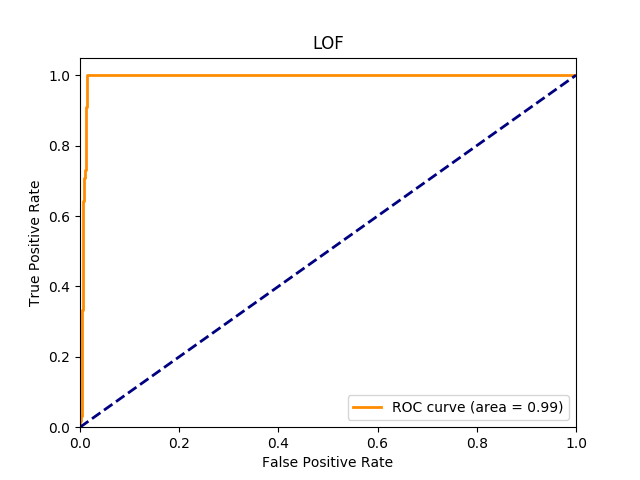
\includegraphics[width=65mm,height=39mm]{imagenes/lof-test.png} }\\
    \multicolumn{2}{c}{Curva ROC para datos reales}
    \end{tabular}
    \caption{\label{fig:loftest} LOF test}
\end{figure}

\begin{figure}[H]
    \begin{tabular}{cc}
      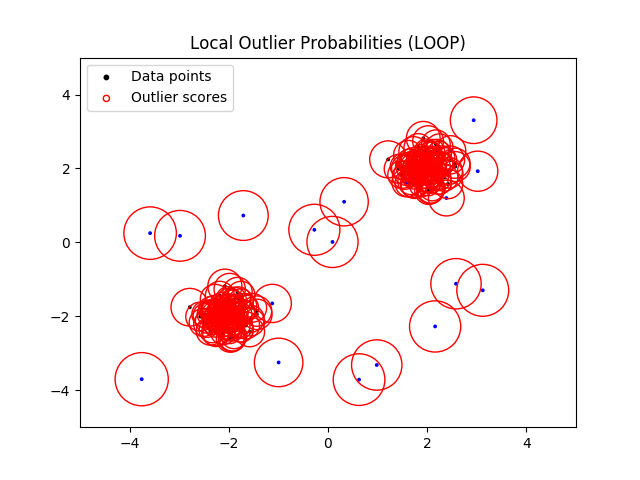
\includegraphics[width=65mm,height=40mm]{imagenes/loop-sintetico.png} &   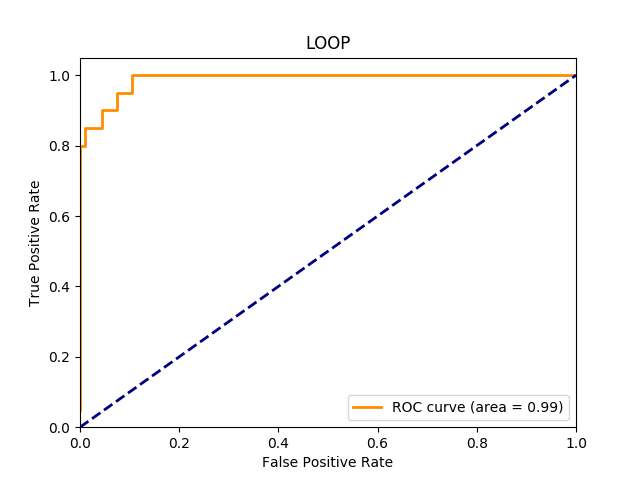
\includegraphics[width=65mm,height=40mm]{imagenes/loop-sintetic-roc.png} \\
    Score & Curca ROC para datos sinteticos \\[6pt]
    \multicolumn{2}{c}{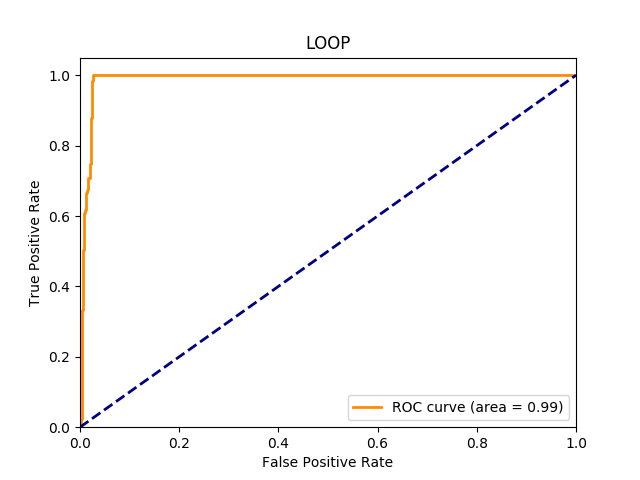
\includegraphics[width=65mm,height=39mm]{imagenes/loop-test.png} }\\
    \multicolumn{2}{c}{Curva ROC para datos reales}
    \end{tabular}
    \caption{\label{fig:looptest} LOOP test}
\end{figure}

\begin{figure}[H]
    \begin{tabular}{cc}
      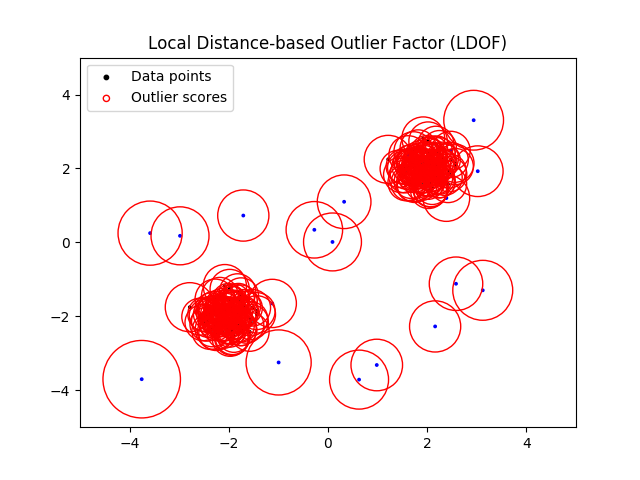
\includegraphics[width=65mm,height=40mm]{imagenes/ldof-sintetico.png} &   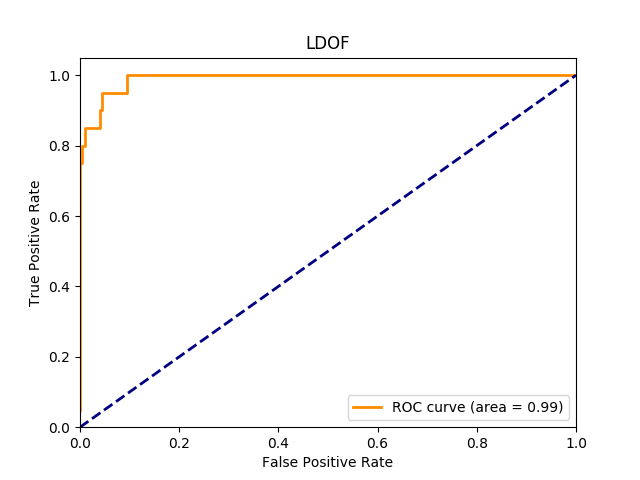
\includegraphics[width=65mm,height=40mm]{imagenes/ldof-sintetic-roc.png} \\
    Score & Curca ROC para datos sinteticos \\[6pt]
    \multicolumn{2}{c}{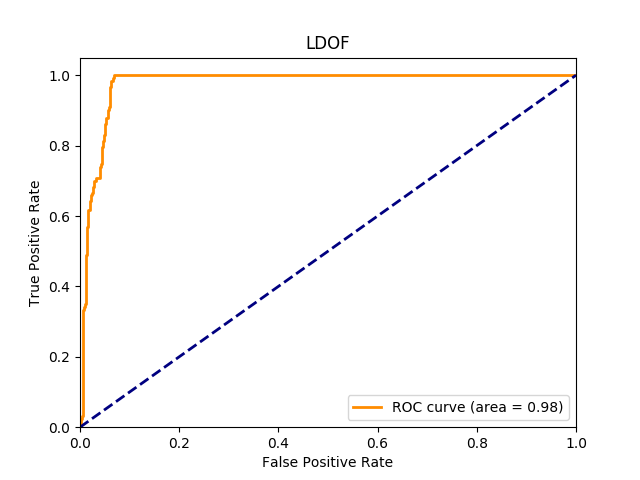
\includegraphics[width=65mm,height=39mm]{imagenes/ldof-test.png} }\\
    \multicolumn{2}{c}{Curva ROC para datos reales}
    \end{tabular}
    \caption{\label{fig:ldoftest} LDOF test}
\end{figure}

\begin{figure}[H]
    \begin{tabular}{cc}
      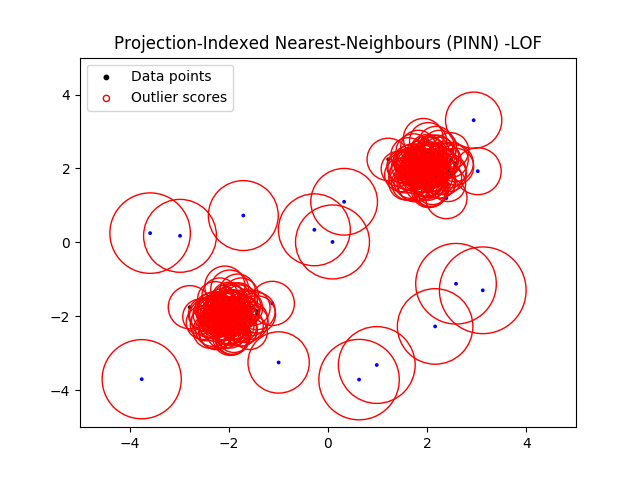
\includegraphics[width=65mm,height=40mm]{imagenes/pinn-lof-sintetico.png} &   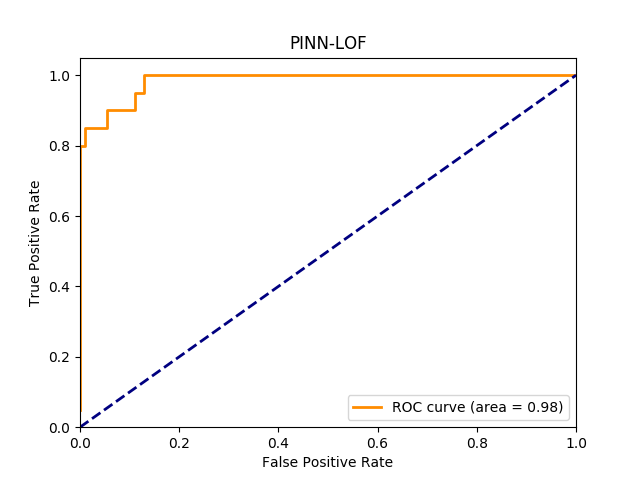
\includegraphics[width=65mm,height=40mm]{imagenes/pinn-lof-sintetic-roc.png} \\
    Score & Curca ROC para datos sinteticos \\[6pt]
    \multicolumn{2}{c}{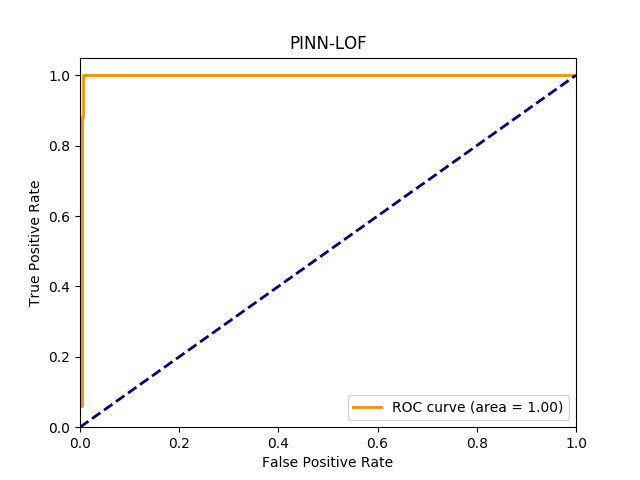
\includegraphics[width=65mm,height=39mm]{imagenes/pinn-lof-test.png} }\\
    \multicolumn{2}{c}{Curva ROC para datos reales}\\
    \end{tabular}
    \caption{\label{fig:pinnloftest} PINN-LOF test}
\end{figure}


\begin{figure}[H]
    \begin{tabular}{cc}
      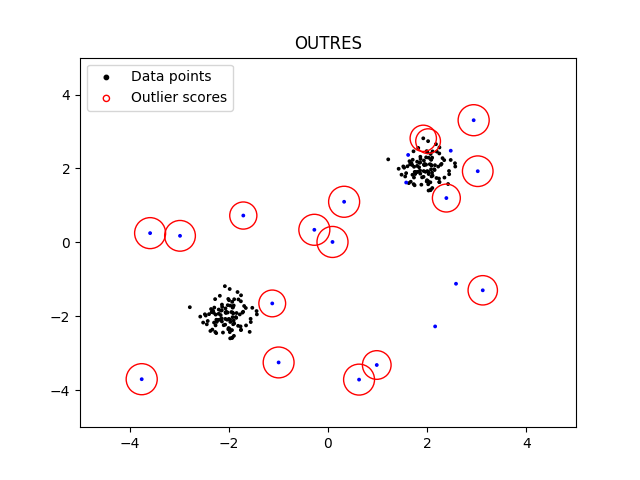
\includegraphics[width=65mm,height=40mm]{imagenes/outres-sintetico.png} &   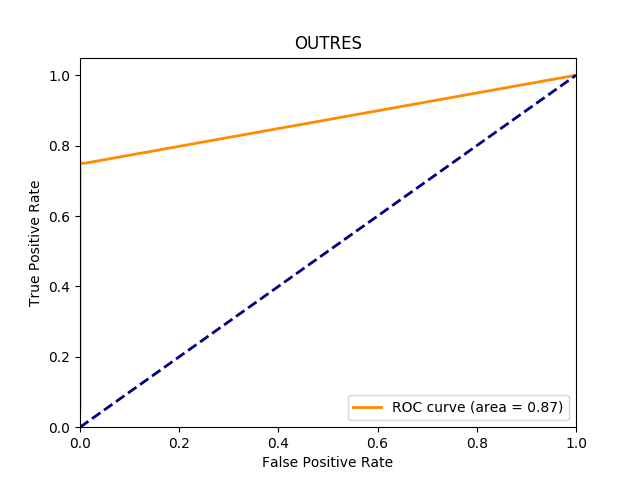
\includegraphics[width=65mm,height=40mm]{imagenes/outres-sintetic-roc.png} \\
    Score & Curca ROC para datos sinteticos \\[6pt]
    \multicolumn{2}{c}{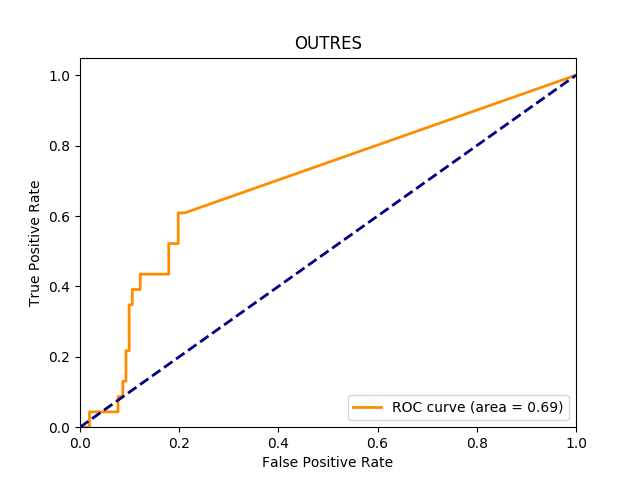
\includegraphics[width=65mm,height=39mm]{imagenes/outres-test.png} }\\
    \multicolumn{2}{c}{Curva ROC para datos reales}\\
    \end{tabular}
    \caption{\label{fig:outrestest} OUTRES test}
\end{figure}

\begin{figure}[H]
  \begin{tabular}{cc}
    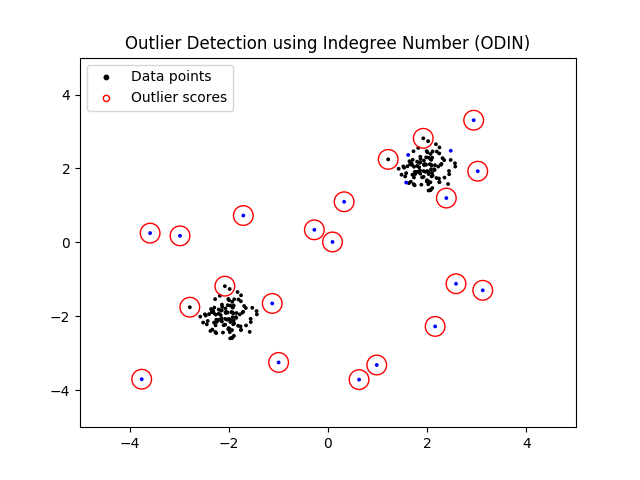
\includegraphics[width=65mm,height=40mm]{imagenes/odin-sintetico.png} &   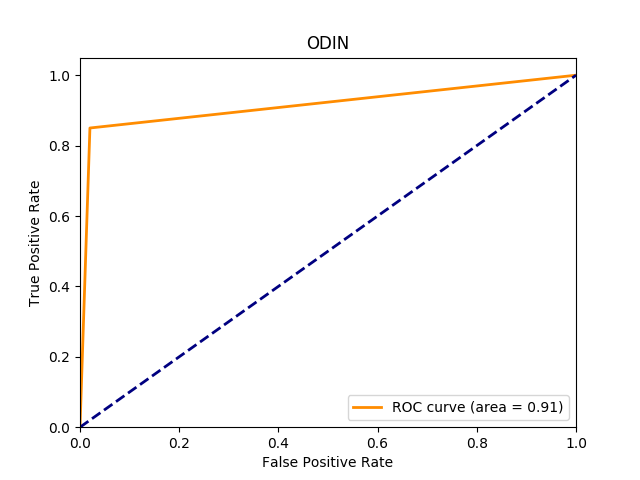
\includegraphics[width=65mm,height=40mm]{imagenes/odin-sintetic-roc.png} \\
  Score & Curca ROC para datos sinteticos \\[6pt]
  \multicolumn{2}{c}{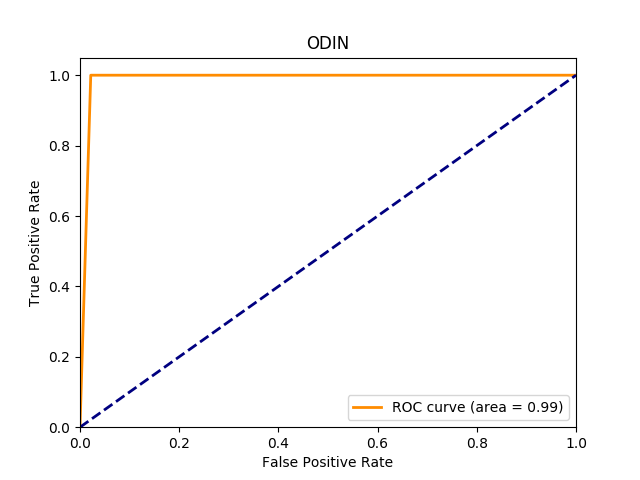
\includegraphics[width=65mm,height=39mm]{imagenes/odin-test.png} }\\
  \multicolumn{2}{c}{Curva ROC para datos reales}\\
  \end{tabular}
  \caption{\label{fig:odintest} ODIN test}
\end{figure}


\begin{figure}[H]
  \begin{tabular}{cc}
    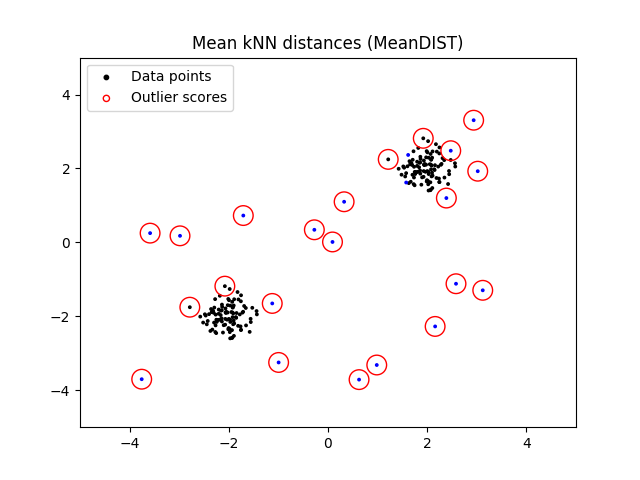
\includegraphics[width=65mm,height=40mm]{imagenes/meandist-sintetico.png} &   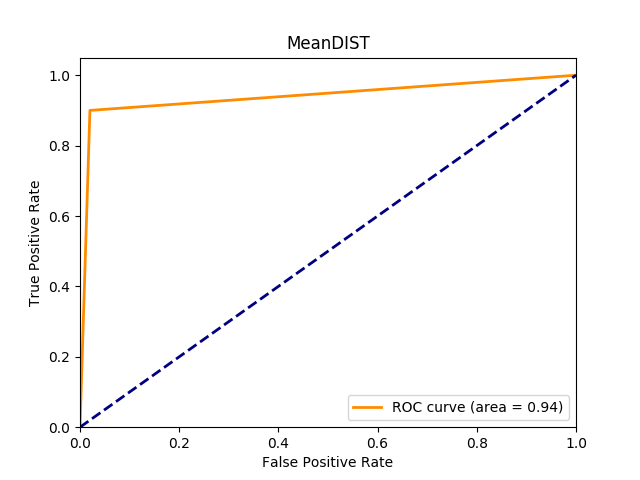
\includegraphics[width=65mm,height=40mm]{imagenes/meandist-sintetic-roc.png} \\
  Score & Curca ROC para datos sinteticos \\[6pt]
  \multicolumn{2}{c}{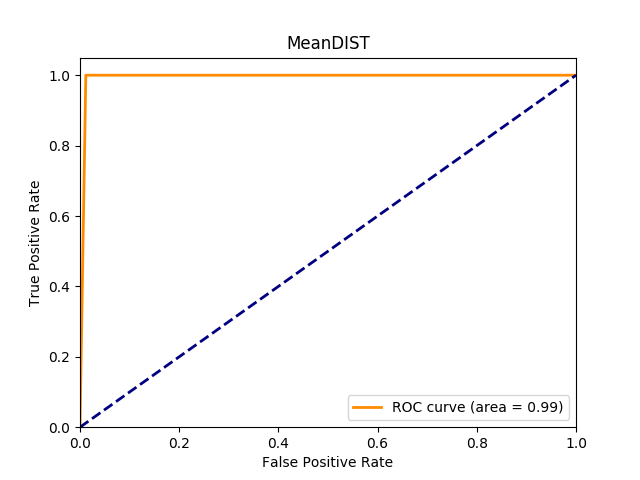
\includegraphics[width=65mm,height=39mm]{imagenes/meandist-test.png} }\\
  \multicolumn{2}{c}{Curva ROC para datos reales}\\
  \end{tabular}
  \caption{\label{fig:meandisttest} MeanDIST test}
\end{figure}

\begin{figure}[H]
  \begin{tabular}{cc}
    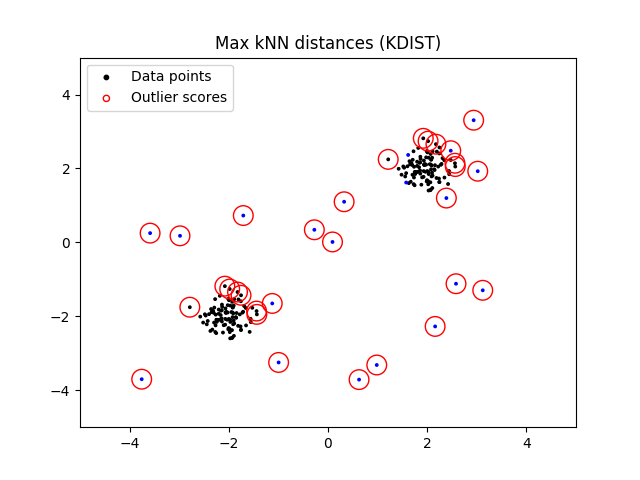
\includegraphics[width=65mm,height=40mm]{imagenes/kdist-sintetico.png} &   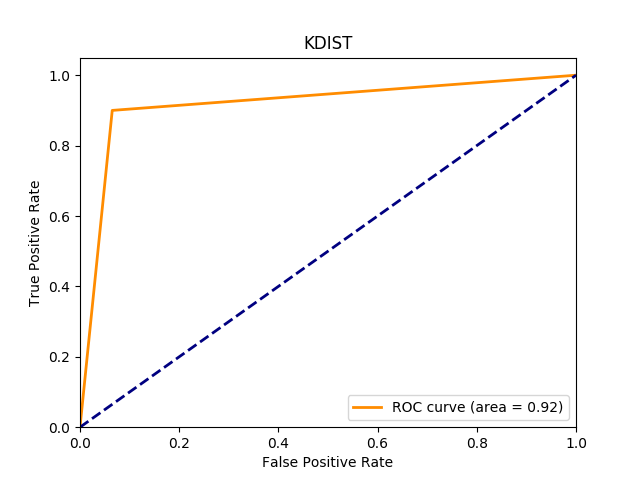
\includegraphics[width=65mm,height=40mm]{imagenes/kdist-sintetic-roc.png} \\
  Score & Curca ROC para datos sinteticos \\[6pt]
  \multicolumn{2}{c}{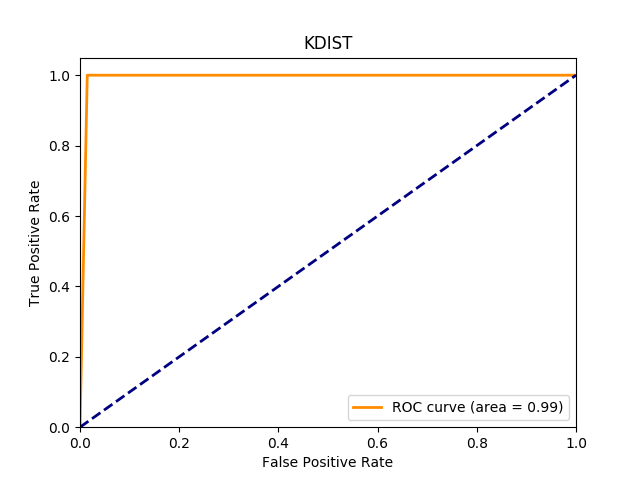
\includegraphics[width=65mm,height=39mm]{imagenes/kdist-test.png} }\\
  \multicolumn{2}{c}{Curva ROC para datos reales}\\
  \end{tabular}
  \caption{\label{fig:kdisttest} kDIST test}
\end{figure}

Como podemos tanto en los datos sintéticos como en el conjunto de datos reales
que hemos utilizado para probar nuestros algoritmos, los resultados son
muy buenos. Todos como podemos ver detectan casi todas las anomalías 
dándole una puntuación alta. Esto lo podemos ver en la primera figura 
donde el radio de los puntos azules, que son las anomalías, son mucho más
amplios que el resto de puntos concentrados en dos grupos.

Para reafirmar la idea tenemos la curva ROC y el área baja la curva que
determina la métrica AUC. Como podemos ver en la mayoría de casos La métrica nos 
indica que los resultados son muy buenos y que tenemos unos buenos métodos para afrontar
el problema.

Quizás podríamos pensar que esto son buenos resultados ya que usamos datos 
sintéticos. Para ello hemos cogido un conjunto de datos aleatorio del repositorio del
que disponíamos para experimentar que comentaremos más adelante. El conjunto de
datos se llama \textit{shuttle-c0-vs-c4.dat} y está compuesto por 9 variables enteras.
De este modo también probamos su correcto funcionamiento en casos más complejos.
Los resultados de dichas pruebas los tenemos en la tercera figura correspondiente a cada
algoritmo. Como podemos ver los resultados obtenidos en los datos sintéticos se mantienen,
y seguimos teniendo unos resultados fantásticos.

La sorpresa para nosotros llegó con el mal desempeño de \textbf{OUTRES}. En primer lugar
tenemos que comentar que a pesar de conocer el hecho de su alta complejidad lo que podía
suponer un alto coste en tiempo, confiábamos en que la técnica de poda hiciera este algoritmo
útil ya que el procedimiento y técnica tenían una idea buena. En la práctica esta idea 
para la cual se realiza la poda, no tiene una buena utilidad. Esto se debe a que en datos 
reales la poda es difícil de realizar ya que es fácil que el test estadístico falle. A pesar de
subir el umbral intentado subir la poda sigue siendo costoso y se aumenta demasiado la poda, los
resultados empeoran. Por tanto, el algoritmo no solo es costoso en tiempo, sino que, además
es complicado conseguir un buen ajuste de los parámetros. Pero en realidad, los
resultados no son competitivos con el resto de algoritmos en este tipo de casos. A pesar de las pruebas
decidimos mantener este algoritmo ya que, aunque en nuestros conjuntos de datos no tenía los mejores factores 
para favorecer su mejor desarrollo, puede que a los usuarios futuros que utilicen
esta herramienta, le ayude y sea un algoritmo que, si se cumplen determinadas condiciones, su comportamiento
sea mejor incluso que los del resto. Este mejor comportamiento lo plantean los autores en 
\cite{mullerAdaptiveOutliernessSubspace2010}. 


En definitiva, podemos ver como nuestra biblioteca
puede afrontar y resolver el problema de la detección de anomalías
desde el enfoque de técnicas basadas en la proximidad. En cuanto a la implementación
de los algoritmos seleccionados queda demostrado que es correcta y robusta.




\section{Experimentación}
En este punto del trabajo ya disponemos de la funcionalidad de nuestra biblioteca por lo que 
una vez que hemos ejemplificado el uso de los algoritmos, realizamos una experimentación 
para probar el comportamiento de nuestros algoritmos frente a 
una gran batería de conjuntos de datos. Con ello obtendremos una gran información y demostraremos 
el desempeño y la robustez de nuestro proyecto. Para ello hemos seleccionado conjuntos de clasificación 
binaria muy desbalanceada con ratios mayores que 9. En los problemas desbalanceados
lo que tenemos es una clase con un número muy pequeño de instancias con respecto
a la clase mayoritaria. El ratio es la relación entre el número de datos de una clase y
la minoritaria. Usamos este tipo de problemas porque, a diferencia de entornos puramente no
supervisados, en este caso disponemos de las etiquetas que usaremos, no para entrenar sino 
para medir el desempeño de los algoritmos. Además, tomamos este tipo de conjuntos de datos 
muy desbalanceados porque esperamos que las anomalías representen un porcentaje pequeño del 
número total de instancias.


Por tanto, la clase minoritaria se tomará como 
anomalías y la clase mayoritaria serán los casos normales de funcionamiento. 
Para medir el desempeño de cada algoritmo usaremos como en el apartado anterior la 
métrica \textbf{AUC} la cual nos ofrece una buena medida sobre el funcionamiento  
de nuestra biblioteca frente a los diversos problemas. 

Para cada algoritmo y cada conjunto de datos se ha realizado una búsqueda de los mejores
parámetros para buscar una puntuación adecuada. En el caso de \textbf{OUTRES}  y la 
complejidad hace inaccesible su uso para conjuntos de datos reales, por lo que no se 
han podido obtener resultados con este algoritmo. Los tiempos de ejecución son realmente
elevados por lo que realizar una busqueda de hiperparámetros y conseguir resultados se
convierte en algo inviable.



Como comentábamos en la introducción existe una biblioteca llamada \textbf{PyOD} 
\cite{zhaoPyODPythonToolbox2019} \cite{zhaoPythonToolboxScalable2019} 
que también implementa algunos algoritmos basados en proximidad, nuestra intención es usar el 
algoritmo \textbf{LOCI} \cite{papadimitriouLOCIFastOutlier2003} de dicha biblioteca  
para comparar los resultados con los nuestros y ver si nuestra biblioteca es competitiva.
Cabe destacar que la execución de \textbf{LOCI}, superaba con diferencia el tiempo de ejecución
de nuestros algoritmos. Para aclarar este punto exponemos nuestra experiencia en la 
experimentación. Si se ejecutaban todos los algoritmos, excepto \textbf{LOCI}, el tiempo de ejecución
era de 20 minutos. En caso de calcular los resultados de \textbf{LOCI}, fueron necesarios más de 2
días.
Esto confirma la idea de que nuestra biblioteca es competitiva en lo que se refiere a velocidad
y tiempo de computación.


Se han seleccionado 20 conjuntos de datos de la base de datos KEEL \cite{alcala-fdezKEELSoftwareTool2009} 
de donde hemos seleccionado un paquete de clasificación binaria muy desbalanceada. La ratio de  
desbalanceo en todos los casos es mayor que 9 y en algunos casos llega a más de 30. Por tanto, 
lo que hemos hecho ha sido tomar como anomalías la clase menos numerosa y el resto de ejemplos 
serán la clase normal. Con esta batería de conjuntos de datos será con la que experimentemos. 

Vamos a ver los resultados obtenidos en la siguiente tabla y los comentaremos posteriormente:

\begin{figure}[h]
  \center{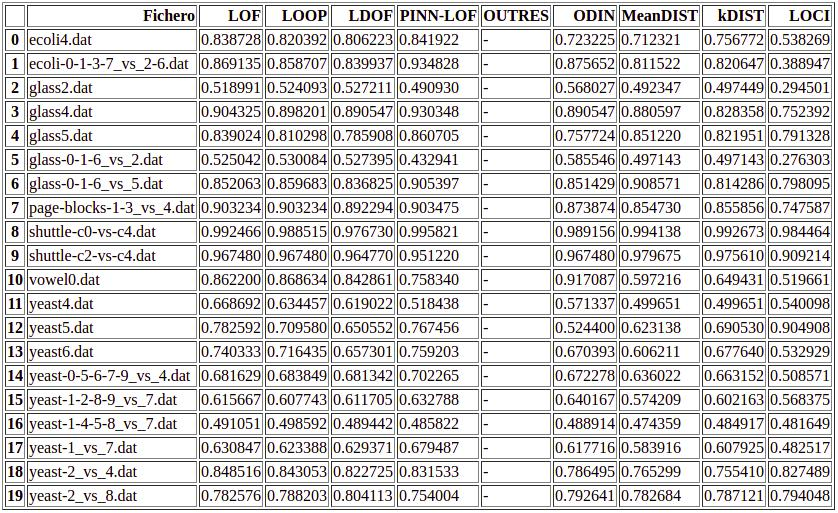
\includegraphics[width=\textwidth]
  {imagenes/resultados.jpeg}}
  \caption{\label{fig:resultados} Valores AUC de la experimentación}
\end{figure}

Como podemos ver en general los resultados son muy variados y fuertemente dependientes del conjunto
de datos al que se enfrenta. Vamos a comentar ciertas cosas que consideramos ciertamente 
interesantes.

En primer lugar, podemos ver como los resultados entre los 6 algoritmos de nuestra biblioteca
 son similares en cada conjunto de 
datos. En primer lugar tenemos que mencionar que en general \textbf{LDOF} no consigue mejores  
resultados que el resto de algoritmos en ningún conjunto de datos. A pesar de ello tampoco podemos 
considerar que obtenga resultados malos ya que está cerca del resto. Esto se debe a que  
\textbf{LDOF} está enfocado a conjuntos de datos dispersos y en nuestro caso teníamos como 
experimentación datos que anteriormente eran considerados una clase, por lo que es fácil suponer 
que entre una parte de los datos considerados anomalías podrían estar agrupados. Esto ha perjudicado 
un poco a \textbf{LDOF}. 

En segundo lugar podemos destacar el comportamiento de \textbf{PINN-LOF}. Su comportamiento es muy positivo
ya que en muchos casos, podemos observar cómo se cumple la necesidad de explorar subespacios. 
Como comentábamos en las explicaciones los algoritmos usan la distancia entre todas las dimensiones, 
esto hace que la diferencia se homogenice cuando realmente la anomalía se diferencia en una o varias subdimensiones. 
Con \textbf{PINN-LOF} seleccionamos subespacios aleatoriamente y se analiza si puede determinarse si es anomalía. 
en casos como en \textbf{ecoli-0-1-3-7-vs2-6, glass4, glass-0-1-6-vs-5} podemos ver que la ganancia es considerable 
con el resto de algoritmos. En algunos casos la ganancia es de $0.1$. Esto se debe a que en esa búsqueda aleatoria 
a través de los distintos subespacios, el algoritmo encuentra un subespacio donde es más fácil 
diferenciar las anomalías. Como podemos ver este enfoque nos puede aportar una mejora considerable. 
También se confirma las sospechas de que a mayor dimensionalidad las diferencia entre distancias se pierde 
ya que en este caso tenemos unos de los conjuntos con más dimensiones del conjunto.
Además, permite una aplicación de \textbf{LOF} de forma más eficiente al no usar todas las dimensiones.
La parte negativa de este algoritmo la encontramos en ejemplos como \textbf{yeast4}. Donde encontramos 
un resultado peor comparado con otros algoritmos. Esto se debe a la búsqueda aleatoria lo que en este 
caso ha propiciado un peor resultado por la elección de subespacios no muy buenos. Debemos  
mencionar que en las pruebas realizadas hemos observado que es un algoritmo totalmente dependiente de  
la aleatoriedad ya que depende totalmente de las elecciones que realiza. Influye más la aleatoriedad 
que los parámetros y ha sido difícil encontrar los parámetros correctos. 

Ahora vamos a analizar los resultados en conjunto de \textbf{LOF y LOOP} ya que se basaban 
en conceptos similares. Como podemos ver esto se ha reflejado en resultados similares. No existe 
una diferencia clara entre ambos algoritmos y los resultados en casi todos los casos son similares. 
Cabe resaltar que de forma general \textbf{LOF} consigue siempre una pequeña mejora que en algunos 
casos. Si se hace notable en algunos conjuntos como en \textbf{yeast5}. Como comentábamos y explicábamos anteriormente  
son algoritmos basados en conceptos similares. La gran ventaja de \textbf{LOOP} es que nos ofrece 
como resultado una probabilidad, lo que facilita su interpretabilidad y la comparación con otros  
algoritmos. 

En cuanto al comportamiento de \textbf{ODIN} podemos decir que realiza un desempeño notable. en general 
obtiene resultados muy similares al resto de algoritmos y en casos como en el conjunto de datos de  
\textbf{vowel0} se consigue un resultado mejor. En definitiva, es un algoritmo con un muy buen 
desempeño. El único inconveniente que podemos poner a este algoritmo es la elección 
de hiperparámetros, ya que el parámetro clave es la selección del umbral del grado de vecinos 
recíprocos que permitimos. Esto hace que sea algo más complejo su ajuste porque para un buen ajuste sería necesario 
conocer información adicional del conjunto de datos o una aproximación del número de anomalías que esperamos 
encontrar. 

Analizamos el comportamiento de \textbf{MeanDIST y kDIST} conjuntamente ya que la idea que subyace bajo 
ambos algoritmos es la misma. En primer lugar, debemos mencionar que, aunque su desempeño de forma general 
suele ser más pobre que el resto de algoritmos, aunque muy cerca. También debemos mencionar que existen casos 
en los que se encuentran soluciones realmente destacables en comparación con el resto, como por ejemplo en  
el conjunto \textbf{glass-0-1-6-vs-5} donde se alcanza una puntuación de. Por tanto, son algoritmos 
que, a pesar de usar una idea más simple para detectar anomalías, existen casos en los que presentan una ventaja 
y no pueden ser descartados. Por otro lado, en este caso se reafirma la idea de que los algoritmos estan condicionados 
al conjunto de datos. Como podemos ver no podemos decir que sea mejor usar la media de distancias o la distancia mayor 
ya que existen casos para los cuales uno tiene un mejor desempeño que el otro. En estos algoritmos nos ha sorprendido 
como un enfoque tan sencillo puede conseguir resultados bastante buenos, aunque queda claro que si queremos 
ser más precisos y conseguir resultados mejores, son enfoques que pueden no ser suficientes. 

Por otro lado, nos deja un mal sabor de boca el comportamiento de Con \textbf{OUTRES} 
ya que los conceptos en los que se basa son similares a Con \textbf{PINN-LOF}, 
la búsqueda de anomalías en subespacios. En \textbf{PINN-LOF} hemos visto como incluso usando 
una selección aleatoria esto puede generar muy buenos resultados y que realmente es necesaria esa  
búsqueda en subespacios, cuando la dimensión crece, no solo por eficiencia sino también por realizar 
una mejor aproximación. En el caso de \textbf{OUTRES} su parte positiva es a la vez la negativa. Considerábamos 
que era muy interesante al realizar esta búsqueda de subespacios relevantes y que podía generar grandes resultados. 
La realidad es que ese análisis tan exhaustivo lo convierte en un algoritmo con una complejidad inaplicable. 
Cierto es que se diseña un sistema de poda, pero en los ejemplos reales este sistema no consigue una poda necesaria 
para hacer eficiente el algoritmo. 

Por último, tenemos los resultados del algoritmo \textbf{LOCI} procedente de la biblioteca PyOD \cite{zhaoPyODPythonToolbox2019}.
Respecto a esta biblioteca ya comentábamos como nuestra biblioteca tenía un mejor desempeño en cuanto a tiempo de ejecución.
En cuanto a los resultados podemos observar la última columna y comparar con el resto de columnas. Claramente podemos ver que existe
una gran diferencia en la puntuación obtenida. Solo en el archivo \textbf{yeast5} consigue un resultado bastante mejor que el resto de
algoritmos. Como conclusión de esta experimentación podemos confirmar que nuestra biblioteca no es solo competitiva a nivel de tiempos
sino que ofrece unos resultados bastante mejores y que ofrece una solución al problema de la detección de anomalías de calidad.

Como aclaración podemos ver que hay conjuntos de datos en los que ningún algoritmo consigue buenos resultados, por ello 
podemos considerar que esto se debe a los datos subyacentes y que realmente sea complicado una separación entre 
anomalías y datos normales. 

Como conclusión final de esta experimentación podemos decir que por un lado tenemos a \textbf{LOF y LOOP}, 
dos algoritmos con muy buenos resultados y sobre todo estables. Consiguen un rendimiento bueno  
en todos los conjuntos aunque destacar que \textbf{LOF} obtiene un mejor desempeño y \textbf{LOOP} nos 
proporciona una interpretabilidad más fácil. Por otro lado hemos analizado el comportamiento de \textbf{LDOF} 
que en general también consigue buenos resultados, aunque no destaca ya que está diseñado para conjuntos de datos 
más dispersos. También tenemos \textbf{PINN-LOF} un algoritmo capaz de conseguir mejores resultados que el resto aunque 
muy inestable por su componente aleatoria. Por último tenemos \textbf{ODIN} el cual nos ofrece muy buenos resultados
pero tiene una mayor complejidad para ajustar los hiperparámetros y \textbf{MeanDIST y kDIST}, algoritmos más simples y 
fáciles de interpretar aunque con un desempeño bueno pero más pobre.


